\documentclass[10pt,a4paper]{article}
%% Language and font encodings
\usepackage[british]{babel}
\usepackage[utf8]{inputenc}
\usepackage[T1]{fontenc}
%% Sets page size and margins
\usepackage[a4paper,top=2cm,bottom=2cm,left=2.5cm,right=2.5cm,marginparwidth=1.5cm]{geometry}
%% Useful packages
\usepackage{amsmath}
\usepackage{graphicx}
\usepackage[colorinlistoftodos]{todonotes}
\usepackage[colorlinks=true, allcolors=blue,]{hyperref}
\usepackage{authblk}
\usepackage[backend=biber,style=numeric-comp]{biblatex}
\usepackage{listings}
\usepackage{xcolor}
\usepackage{amsmath} \allowdisplaybreaks% lets align equations break over pages.
\usepackage{amssymb}

\definecolor{codegreen}{rgb}{0,0.6,0}
\definecolor{codegray}{rgb}{0.5,0.5,0.5}
\definecolor{codepurple}{rgb}{0.58,0,0.82}
\definecolor{backcolour}{rgb}{0.95,0.95,0.92}


% \addbibresource{references.bib}

\lstdefinestyle{mystyle}{
  backgroundcolor=\color{backcolour}, 
    commentstyle=\color{codegreen},
    keywordstyle=\color{magenta},
    numberstyle=\tiny\color{codegray},
    stringstyle=\color{codepurple},
    basicstyle=\ttfamily\footnotesize,
    breakatwhitespace=false,         
    breaklines=true,                 
    captionpos=b,                    
    keepspaces=true,                 
    numbers=left,                    
    numbersep=5pt,                  
    showspaces=false,                
    showstringspaces=false,
    showtabs=false,                  
    tabsize=2
  }
\lstset{style=mystyle}

\graphicspath{{./img/}}

%% Title
\title{
  {\Huge Simulation and Performance Evaluation}\\
  \huge Homework 1 \\
}

\author{Blascovich Alessio and Di Noia Matteo}

\begin{document}

\maketitle

\section*{Exercise 1}

\begin{center}
  \begin{lstlisting}[language=python]
  def main():
      # Definition of normal distribution parameters
      choice_mean = [-2, 4, 10, 15]
      choice_var = [2, 1, 3, 2]
      choice_prob = [0.15, 0.25, 0.35, 0.25]
      vals = []
      
      rng = np.random.default_rng()
      RANGE = 1000000
      for _ in range(RANGE):
          mu, var = choices(list(zip(choice_mean, choice_var)), choice_prob)[0]
          vals.append(rng.normal(mu, np.sqrt(var)))
      print(np.mean(vals))
      print(np.var(vals))
      # [...]
  \end{lstlisting}
\end{center}

This is the simulation we run to firstly extract randomly the normal distribution parameters, line 11, from \texttt{choice\_var} and \texttt{choice\_mean}, with the probability vector \texttt{choice\_prob}. Then we generate a sample from the created normal distribution, this sample is appended to a vector of values collecting all the sampling, The parameters pick and the sampling process was repeated \(1000000\) times. On the resulting vector of values we computed arithmetic mean and arithmetic variance, line 13 and line 14. 

\begin{center}
  \begin{lstlisting}[language=python]
  def compute_mean(values, probs):
      return sum(v * p for v, p in zip(values, probs))
    
  def compute_var(values,  probs):
      squared = map(lambda x: x**2, values)
      return compute_mean(squared, probs) - compute_mean(values, probs)**2
  
  def main():
      # [...]
      print("EXPECTED ARE:")
      expected_mean = compute_mean(choice_mean, choice_prob)
      expected_var = (compute_var(choice_mean, choice_prob)
                   + compute_mean(choice_var, choice_prob))
      print(expected_mean)
      print(expected_var)
  \end{lstlisting}
\end{center}

To validate the result against the expected we computed the theoreticial mean and variance of the conditional distribution. For the expected value we simply used the formula of the conditional mean, meanwhile for the variance we applied the conditional variance formula.

We call \(X\) the random variable obtained by conditioning the normal distribution parameters with probability vector given.
\begin{align*}
  \mathbb{E}[X] &= \sum^{4}_{i=1}{\mathbb{E}[X|Y_{i}]P(Y_{i})}\\
  Var(X) &= \mathbb{E}[Var(X|Y)] + Var(\mathbb{E}[X|Y])
\end{align*}

The Python script described above produced:
\begin{center}
  \begin{lstlisting}
    EXPECTED ARE:
    7.95
    34.747499999999995
    COMPUTING...
    7.951787799337237
    34.71597133688908
  \end{lstlisting}
\end{center}
Which leads us to conclude resulting dataset obeys the conditional mean and conditional variance formulae.

\begin{figure}[h]
  \centering
  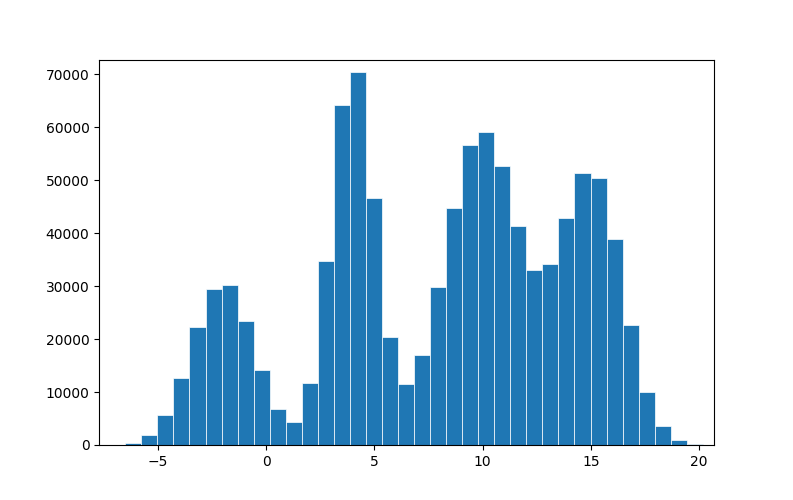
\includegraphics[scale=0.4]{exercise-1-hist.png}
\end{figure}

The plot of the random values obtained during the sampling phase presents four peaks in correspondence of the four normal means and the height of these peaks is proportional to the probability of choosing that distribution parameters.
\section*{Exercise 2}
\begin{center}
  \begin{lstlisting}[language=python]
    RANGE = 1000000
    vals_exp: list = []
    vals_uni: list = []
    rng = np.random.default_rng()
    
    # Generate 1M random value of exponential and uniform
    for _ in range(RANGE):
    vals_exp.append(rng.exponential(1))
    vals_uni.append(rng.uniform(0, 5))
    
    # Count how many exponential are grater than the corresponding uniform
    greater = sum(1 for i in range(RANGE) if vals_exp[i] > vals_uni[i])
    print(greater / RANGE)
  \end{lstlisting}
\end{center}
We used the above code to generate \(1000000\) draws from each distribution. We considered \(1000000\) an acceptable sample size since it was the same size suggested by the professor to obtain statisticial meaningful data in exercise 1.  Then, we counted how many exponential draws were larger that the corresponding uniform draw. The result was then divided by the length of the dataset to obtain the probability for which the exponential random variable is greater that the uniform random variable. In our tests the probability was \(0.198286\).

\begin{figure}[h]
  \centering
  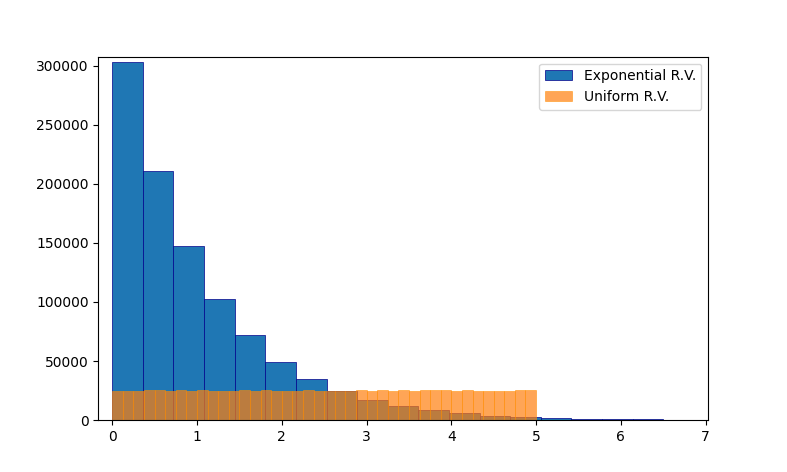
\includegraphics[scale=0.4]{exercise-2-hist.png}
\end{figure}

\subsection*{Facultative}

Let \(X\sim\text{Exp}(\lambda = 1)\) and let \(Y\sim U(0,5)\), this exercise ask to quantify \(P(X>Y)\). We have:
\begin{align}
  \label{eq:1.1}
  f_{X}(x) = e^{-x} \quad\textrm{and}\quad F_{X}(x) = 1 - e^{-x} \quad&\textrm{with}\quad x\in\left[0,\infty\right)\\
  \label{eq:1.2}
  f_{Y}(y)=\frac{1}{5} \quad\textrm{and}\quad F_{Y}(y) = \frac{y}{5}\quad&\textrm{with}\quad y\in\left[0, 5\right]
\end{align}
We can now define:
\begin{equation*}
  P(X>Y) = \int^{5}_{0}{P(X>y)F_{Y}(y)dy} + \int^{\infty}_{5}{f_{X}(x)dx}
\end{equation*}
Our goal can be decompose in, the probability that \(X\) is greater than a given value \(y\) plus the probability that the exponential random variable has a value greater than \(5\). We can simply the above formula using the definition of probability and the definitions in~\ref{eq:1.1} and~\ref{eq:1.2}.
\begin{equation}
  \label{eq:2}
  P(X>Y) = \int^{5}_{0}{(1 - F_{X}(y))\frac{y}{5}}dy + (1 - F_{X}(5)) = \int^{5}_{0}{e^{-y}\frac{y}{5}}dy + e^{-5}
\end{equation}
Solving the first integral by part we obtain:
\begin{equation*}
  \frac{1}{5}\int^{5}_{0}{ye^{-y}}dy = \frac{1}{5}\left[-ye^{-y} + \int{e^{-y}}dy\right]_{0}^{5} = \frac{1}{5}\left[-ye^{-y} - e^{-y}\right]_{0}^{5} = \frac{1-6e^{-5}}{5}
\end{equation*}
Applying the above result to~\ref{eq:2}, the aimed probability results in:
\begin{equation*}
  P(X>Y) = \frac{1-6e^{-5}}{5} + e^{-5} \approx 0.19865 
\end{equation*}
This calculated value is in line with the experimental value.
\end{document}
